\documentclass[twoside]{article}

\usepackage[math]{kurier}
\usepackage[sc]{mathpazo}
\usepackage{graphicx}
\usepackage{subcaption}
\usepackage{algorithm}
\usepackage[noend]{algpseudocode}
\renewcommand{\sfdefault}{kurier}
\usepackage{color,soul}
\usepackage{amsmath}
\usepackage{graphics}
\setlength{\oddsidemargin}{0.25 in}
\setlength{\evensidemargin}{-0.25 in}
\setlength{\topmargin}{-0.6 in}
\setlength{\textwidth}{6.5 in}
\setlength{\textheight}{8.5 in}
\setlength{\headsep}{0.75 in}
\setlength{\parindent}{0 in}
\setlength{\parskip}{0.1 in}

\makeatletter
\def\BState{\State\hskip-\ALG@thistlm}
\makeatother


\newcounter{lecnum}
\renewcommand{\thepage}{\thelecnum-\arabic{page}}
\renewcommand{\thesection}{\thelecnum.\arabic{section}}
\renewcommand{\theequation}{\thelecnum.\arabic{equation}}
\renewcommand{\thefigure}{\thelecnum.\arabic{figure}}
\renewcommand{\thetable}{\thelecnum.\arabic{table}}


\newcommand{\lecture}[3]{
   \pagestyle{myheadings}
   \thispagestyle{plain}
   \newpage
   \setcounter{lecnum}{#1}
   \setcounter{page}{1}
   \noindent
   \begin{center}
   \framebox{
      \vbox{\vspace{2mm}
    \hbox to 6.28in { {\bf \sffamily AA 274: Principles of Robotic Autonomy
                        \hfill Winter 2019} }
       \vspace{4mm}
       \hbox to 6.28in { {\sffamily{\Large \hfill Lecture #1: #2  \hfill}} }
       \vspace{2mm}
      \vspace{2mm}}
   }
   \end{center}
   \markboth{Lecture #1: #2}{Lecture #1: #2}

   \vspace*{4mm}
}


%%% bibliography configuration %%%
\renewcommand\refname{\hfil Further Reading}
\bibliographystyle{unsrt}

% Aristos Athens
\usepackage{filecontents}
\begin{filecontents}{biblio.bib}
@article{lavalle2001randomized,
  title={Randomized kinodynamic planning},
  author={LaValle, Steven M and Kuffner Jr, James J},
  journal={The international journal of robotics research},
  volume={20},
  number={5},
  pages={378--400},
  year={2001},
  publisher={SAGE Publications}
}
@article{janson2018deterministic,
  title={Deterministic sampling-based motion planning: Optimality, complexity, and performance},
  author={Janson, Lucas and Ichter, Brian and Pavone, Marco},
  journal={The International Journal of Robotics Research},
  volume={37},
  number={1},
  pages={46--61},
  year={2018},
  publisher={SAGE Publications Sage UK: London, England}
}
@article{jahanshahi2019robot,
  title={Robot Motion Planning in an Unknown Environment with Danger Space},
  author={Jahanshahi, Hadi and Jafarzadeh, Mohsen and Sari, Naeimeh Najafizadeh and Pham, Viet-Thanh and Huynh, Van Van and Nguyen, Xuan Quynh and others},
  journal={Electronics},
  volume={8},
  number={2},
  pages={201},
  year={2019},
  publisher={Multidisciplinary Digital Publishing Institute}
}
@article{hsu1999path,
  title={Path planning in expansive configuration spaces},
  author={Hsu, David and Latombe, Jean-Claude and Motwani, Rajeev},
  journal={International Journal of Computational Geometry \& Applications},
  volume={9},
  number={04n05},
  pages={495--512},
  year={1999},
  publisher={World Scientific}
}
\end{filecontents}


%%%%%%%%%%%%%%%%%%%%%%%%%%
%document
\begin{document}
%modify this
\lecture{16}{Sampling-based motion planning}{} % Javier Sagastuy

\section{Introduction}
During this lecture we continue our survey of motion planning algorithms and focus mostly on state of the art motion planning algorithms.
Please see Chapter 5 of \textit{Planning Algorithms} by Steven Lavelle for more information about these class of algorithms.

Recall, the purpose of sampling-based motion planning is to find an action trajectory $\textbf{u}(t)$ yielding a feasible $\textbf{x}(t) \in X_{free}$ over time horizon $t \in [0, T]$ which satisfies $\textbf{x}(t) \in X_{goal}$ and minimizes \[
J = \int_0^T g(\textbf{x}, \textbf{u}) dt
\]

This is so say, we want to find a path from our initial state to a goal region that avoids obstacles and possibly optimizes cost (such as trading off time with control effort).
The reason this task is so difficult for mobile robots is that one cannot compute the minimum of $J$ online.
We therefore need to develop very fast algorithms that can be repeatedly computed on-the-fly as the robot explores its environment.

One way to do this is to only consider "snap-shots" of the problem within a short horizon: plan a route, move, re-plan, move again, and so on.
In this case, the short-term goal regions are waypoints along a longer path to the ultimate goal and we only plan a portion of this larger route at a time.
This reduces the amount of data to compute and allows the environment to change between steps.

We'll begin by covering the \textit{configuration space}.
The main is that the motion planning problem is easily described in the real-world, but in reality, it lives in another space: the configuration space.
The following section explores the configuration space and how and why it is useful to solve this problem.

As we had probably mentioned before, there are two main approaches to motion planning:
\begin{itemize}
  \item \textit{Combinatorial planning}: These type of algorithms construct structures in the configuration space that discretely and completely capture all the information needed to plan motion.
  \item \textit{Sampling-based planing}: This approach uses collision detection algorithms to probe and incrementally search the configuration space for a solution, rather than attempting to completely characterize the free space.
\end{itemize}

This lecture we'll focus on the latter class of motion-planning algorithms, rather than seeking to construct a discrete representation that will exactly capture a solution, as we did during the last lecture.
The type of motion planning algorithms that we'll study in this lecture are conceptually very simple, flexible and fairly easy to implement.

As such, we'll complete our survey of sampling based motion-planning algorithms by exploring:
\begin{enumerate}
  \item The Geometric Case
  \item The Kinodynamic Case
  \item Deterministic Samples
  \item Conclusions on motion planning
\end{enumerate}

The key learning objectives for this lecture are:
\begin{itemize}
  \item To understand the configuration space formulation of the motion planning problem and the utility of casting the problem in this space rather than in the real world.
  \item To understand the difference between combinatorial algorithms and sampling based motion planning algorithms, as well as pros and cons of the latter.
  \item To explore a few different cases of sampling based algorithms, understanding their components and theoretical properties (completeness, quality, robustness).
\end{itemize}

\section{Configuration Space} % Zachary Blum
The configuration space defines the possible states of a robot.
If a configuration for a given state is possible, it is called \lq\lq free\rq\rq.
The main idea behind motion planning algorithms is to represent the robot as a single point, and in order to guarantee that the computed motion plan occurs only within the free areas of the configuration space, one must enlarge the obstacles.
One commonly used technique to expand the obstacles is to slide the robot\rq s shape around each obstacle by one vertex of the robot.
Figure \ref{fig:2Dslide} shows an example of this technique in two dimensions, where the gray area is the original obstacle region and the pink area is the enlarged obstacle region - the region where the vertex of the robot cannot enter without a collision occurring.
With the enlarged obstacles in the configuration space, a two-dimensional path can be found from start to goal by considering a two-dimensional point instead of an entire object moving about the space.
The set of free poses in the configuration space is denoted $C_{free}$ and the set of poses where an obstacle lies in $C_{obs}$.

\begin{figure}[H]
\centering
\begin{subfigure}[t]{0.49\textwidth}
\centering
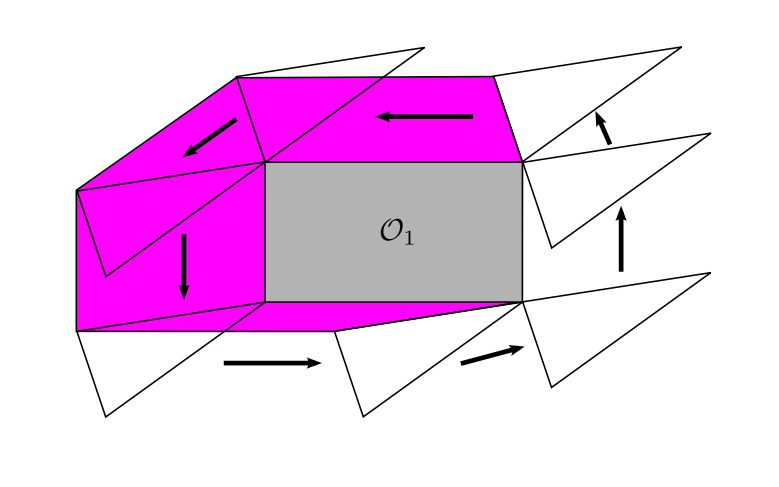
\includegraphics[width=\columnwidth]{SlideRobot1.png}
\caption{}
\end{subfigure}
\hfil
\begin{subfigure}[t]{0.49\textwidth}
\centering
\includegraphics[width=\columnwidth]{SlideRobot2.png}
\caption{}
\end{subfigure}

\caption{(a) Enlarging an obstacle by sliding a triangular-shaped robot around the object by the top-left vertex of the robot. (b) The configuration space with the enlarged obstacles.}
\label{fig:2Dslide}
\end{figure}

This technique works very well for two-dimensions but increases in difficulty with larger dimensions. When considering three dimensions (i.e. two-dimensional position in addition to heading) the configuration space can be built by incrementally fixing the third dimension and enlarging the obstacles in two-dimensions for each increment of the third dimension. This builds layers of the configuration space where each layer is fixed in the third dimension. Figure \ref{fig:3Dslide} shows the steps of building up the configuration space in three-dimensions by incrementally fixing the heading of the robot.

\begin{figure}[H]
\centering
\begin{subfigure}[t]{0.32\textwidth}
\centering
\includegraphics[width=\columnwidth]{3DSlide1.png}
\caption{}
\end{subfigure}
\hfil
\begin{subfigure}[t]{0.32\textwidth}
\centering
\includegraphics[width=\columnwidth]{3DSlide2.png}
\caption{}
\end{subfigure}
\hfil
\begin{subfigure}[t]{0.32\textwidth}
\centering
\includegraphics[width=\columnwidth]{3DSlide3.png}
\caption{}
\end{subfigure}

\caption{(a) Fixing $\theta$ and sliding the obstacle around in a two-dimensional slice of the configuration space. (b) Stacking multiple fixed slices of the configuration space. (c) Continuous representation of the three-dimensional configuration space.}
\label{fig:3Dslide}
\end{figure}

While many robotic applications have two or three dimensional configuration spaces, there are some cases in which a higher dimensional configuration space is required.  One such example is a rigid body in three-dimensional space, which requires a six-dimensional configuration space: three dimensions for x, y, and z position, and three dimensions for the rotations about each of those axes.

An additional useful example of configuration space is the configuration space of a 2R robot arm (two revolute joints). This example (including the figure and caption shown below) is from "Modern robotics: mechanics, planning, and control" by Kevin M. Lynch and Frank C. Park.
\begin{figure}[H]
\centering
\begin{subfigure}[t]{0.20\textwidth}
\centering
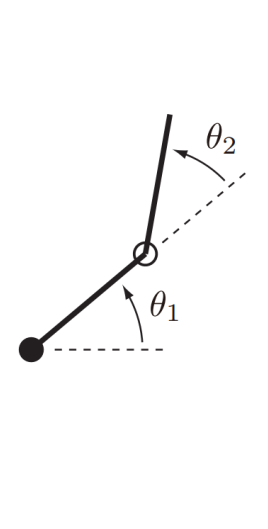
\includegraphics[width=\columnwidth]{ConfigSpaceDiff1.png}
\caption{}
\end{subfigure}
\hfil
\begin{subfigure}[t]{0.39\textwidth}
\centering
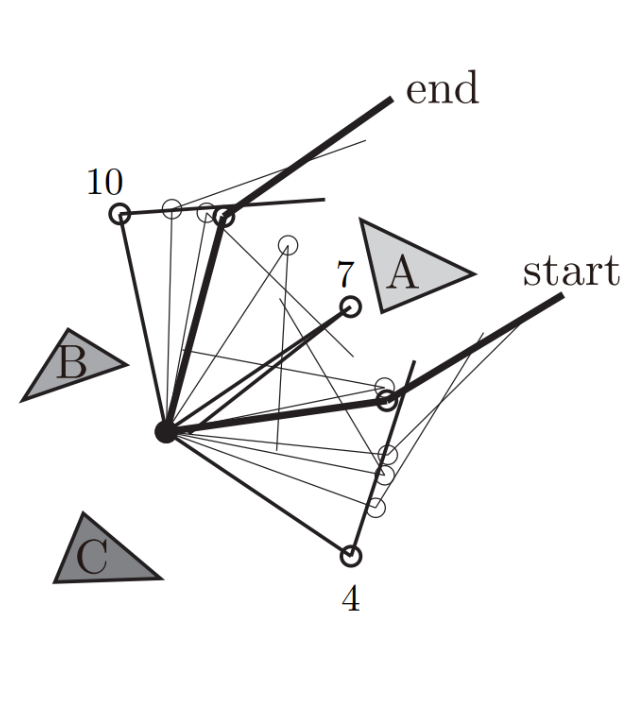
\includegraphics[width=\columnwidth]{ConfigSpaceDiff2.png}
\caption{}
\end{subfigure}
\hfil
\begin{subfigure}[t]{0.39\textwidth}
\centering
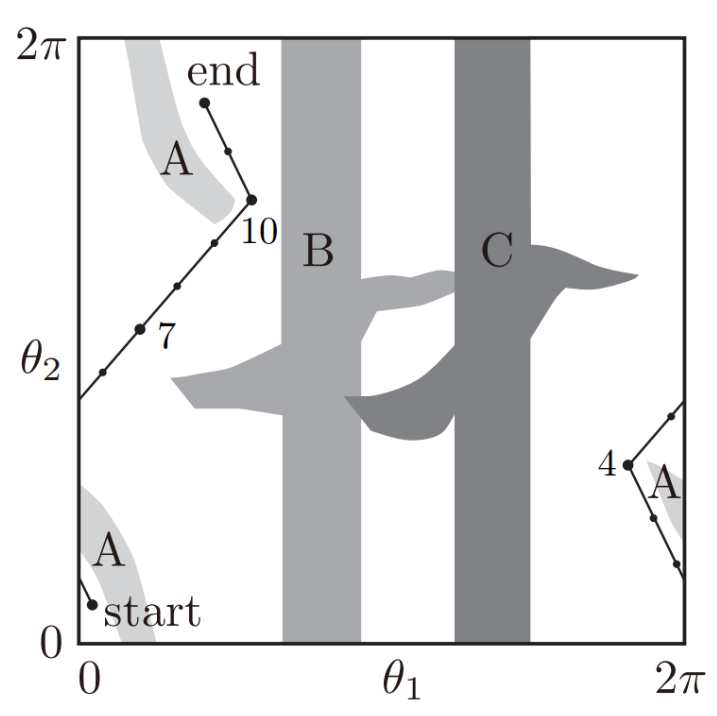
\includegraphics[width=\columnwidth]{ConfigSpaceDiff3.png}
\caption{}
\end{subfigure}

\caption{(a) The 2R robot arm with joint angles shown. (b) The arm navigating in an environment with obstacles A, B , and C in the original robot space.  (c) The arm navigating in an environment with obstacles A, B , and C in the configuration space.}
\label{fig:ConfigSpaceDiff}
\end{figure}

This simple robot, which has two degrees of freedom since the first joint is fixed, is constrained to the environment shown in the middle picture.  The configuration space is shown on the right as a plot of the second joint angle and the first joint angle.  The grey A, B, and C regions shown on this rightmost graph are the obstacles projected into this configuration space.

Since every point in the configuration space maps to a point in the state space of the robot, the configuration space allows the roboticist to determine the states that are free, and will ultimately allow the construction of a path for motion planning.

\subsection{Approaches to motion planning}

Taking a look at Figure \ref{fig:3Dslide}, it becomes fairly apparent that building a configuration space in three or more dimensions can be extremely cumbersome. Once you include kinematic constraints and other restrictions, it becomes very difficult to compute the positions of the obstacles in the state space.

There are two approaches to motion planning: \textit{combinatorial planning} and \textit{sampling based planning}. The former constructs structures in the C-space that discretely and completely capture all information needed to perform planning. In other words, these algorithms construct a discrete representation of the problem that \textit{exactly} captures the solution and they correctly determine in finite time whether or not a solution exists. The latter is a randomized algorithm that uses collision detection algorithms to probe and incrementally search the C-space for a solution, rather than completely characterizing all of the $C_{free}$ structure. The developments of sampling-based approaches was actually stimulated by the limitations of combinatorial approaches. The new creators of the new algorithms chose to abandon the idea of explicitly characterizing $C_{free}$ and $C_{obs}$ and instead capture the structure of C by random sampling. They then use a black-bos component (collision checker) to determine whether the random configuration lies in $C_{free}$ and use a probing scheme to incrementally build a roadmap and then plan a path. Sampling-based algorithms are by far the most common choice for industrial-grade problems as they are conceptually simple, relatively easy to implement, flexible, and can be extended beyond the geometric case. However, it is unclear how many sample should be generated to retrieve solutions and the algorithm is incapable of determining that a solution doesn't exist.

\section{Overview of sampling-based algorithms} % Dikwaka Ganesan
There are two main categories of sampling-based algorithms for motion planning that we will discuss: geometric, and kinodynamic.

\subsection{Basic Components of Sampling Based Algorithms} % Robert Dyro

The two core components of sampling based algorithms are (1) choosing samples in the configuration space in an unstructured way and (2) operating on the connections between samples. The basic realization is that once enough connections between individually samples are made, a path from initial to final state might exist. So long as every connection between each sample is collision free, the entire path is collision free. Points and connections add up to a final motion plan, so they all need to be valid.

In other words, choose points (states) in your configuration space, determine valid connections between them and check if a path from initial to final state exists. Continue picking points until it does or until a prescribed number or time limit. Optionally, ensure that the path is optimal, conditioned on the available connections.

Using unstructured samples, as opposed to a structured choice, does away with the complex task of creating a grid. Some algorithms, like Probabilistic Road Maps and Fast Marching Tree, choose samples first and then create the connections. Some, like Rapidly-exploring Random Trees, choose a sample and make a corresponding connection at the same time. As with Kinodynamic Planning, the connections need not be straight lines, but could be any valid transition paths.

\subsection{Advantages and Disadvantages of Sampling-Based Algorithms} % Ben Kumar
Sampling based methods are used more frequently in industry than combinatorial methods and have an inherent advantage over those methods due to their relative simplicity. Combinatorial approaches attempt to explicitly characterize the configuration space of the problem through methods such as an occupancy grid. Sampling based-methods, on the other hand, create a discrete representation of the problem and can do so while maintaining the accuracy of combinatorial-based methods.

There are a few more advantages of sampling-based methods. The relative simplicity of the algorithm means that they are generally easier to implement. They are also more flexible and can be used in multiple applications with minimal modification. Another advantage is that sampling-based methods can plan paths based on more than just collision avoidance; for instance, they are capable of handling differential constraints, such as for control requirements.

There are a few disadvantages. Sampling-based algorithms need to be run for a finite number of iterations to discover a solution. However, it is not always clear how many iterations are required before a reasonable solution can be obtained. Also, some sampling-based algorithms are not capable of determining if a solution does not exist. However, the fast execution time of these algorithms generally outweigh these minor disadvantages.

\section{Geometric Algorithms}
In the geometric planning case, the system does not have any dynamics, or the dynamics can be solved using a simple integrator. Essentially, one can directly control the pose of the robot as opposed to only the first or second derivative of the pose. There are two main algorithms we have for this case: Probabilistic Roadmap (PRM) algorithms, and Rapidly-exploring Random Trees (RRT) algorithms.

\subsection{Probabilistic Roadmaps}
The key insight of a probabilistic roadmap is to avoid the issue of creating a well characterized configuration space (which is computationally expensive), and simply randomly pick samples in the state space to analyze. At a high level, the algorithm proceeds as follows: First, throw a bunch of random samples into your state space (usually a thousand samples will suffice), discarding forbidden configurations. Then write a collision checker: a computationally cheap algorithm that tests whether the transition between any two samples in the state space results in a collision with an object. Now, the challenge is to connect all the random samples you just generated in some meaningful way. A relatively intuitive technique to doing so is to simply place an arbitrary disk (called the disk connectivity radius) around each sample $x_i$ and add an edge between $x_i$ and all samples that are within the disk and are collision-free. Figure \ref{fig:prm_collision} illustrates this process.

\begin{figure}[H]
  \centering
  \includegraphics[width=50mm]{prm_collision.png}
  \caption{PRM Collision Checking}
  \label{fig:prm_collision}
\end{figure}


After you iterate through all the samples and add all the relevant edges, you should have a graph that extends from $x_{init}$ to $x_{goal}$. You can then use a shortest-path algorithm like $A^*$ to compute the optimal path from the starting pose to the goal pose.

There is a caveat to PRM: while it tends to provide a good characterization of the state space you need to perform many costly collision checks. During each check he PRM algorithm attempts to connect a new node in the state space with all potential neighbors, which can add up.

\subsection{Rapidly-exploring Random Trees}
The Rapidly-exploring Random Trees (RRT) algorithm was developed to respond to the issues with Probabilistic Roadmaps. As discussed, PRMs produce high quality motion plans but use a very dense characterization of the state space to do so. RRT on the other hand, is a lightweight approach. Rather than attempting to characterize the entire state space we attempt to build a \lq\lq portfolio\rq\rq of trajectories incrementally as the algorithm progresses.

Suppose you have already somehow developed two trajectories as seen in Figure \ref{fig:rrt_portfolio}.

\begin{figure}[H]
  \centering
  \includegraphics[width=50mm]{rrt_portfolio_of_trajectories.png}
  \caption{Initial \lq\lq portfolio\rq\rq\ of trajectories}
  \label{fig:rrt_portfolio}
\end{figure}

Notice that this portfolio is incomplete - we are trying to expand it to get to our goal region. At each step of the algorithm, we randomly generate a new sample in the state space, Figure \ref{fig:rrt_new_sample}.

\begin{figure}[H]
  \centering
  \includegraphics[width=50mm]{rrt_new_sample.png}
  \caption{RRT New Sample}
  \label{fig:rrt_new_sample}
\end{figure}

We must then connect this sample to our tree. There are a variety of strategies we can use, but the simplest is to connect the new node to the closest node already on the graph. We keep repeating this process until we reach the goal region.

As you may have noticed, the quality of paths that RRT produces can be quite poor. There is an improved method called RRT* that includes an optimization scheme to improve upon RRT.

In RRT*, we can first try to optimize the way we connect a random new node $x_i$ to our graph. After we find the node $x_{near}$ in the graph, we can analyze the neighbors of $x_{near}$ to see if there is a cheaper way to connect $x_i$ to the graph. This method introduces a notion of local optimality to the algorithm. We can also check if it is possible to get to any of the neighbors of $x_near$ faster if we were to go through $x_i$. Again, remember we must be using the collision checker each time we add an edge to the graph.

RRT algorithms find a feasible path very quickly, but these paths can often be sub-optimal. If one bad step is taken along the way there is nothing in the RRT algorithm that discourages the exploration of long paths.

\subsection{Fast Marching Tree Algorithm (FMT*)} % Yiwei Zhao
Ideally, we want to combine the features of both single-query algorithms (chiefly RRT, which is quick but poor) and multiple-query algorithms (chiefly PRM, which requires a large number of costly collision checks). One way is to run a dynamic programming algorithm called the Fast Marching Tree Algorithm (FMT*) on sample nodes in a way that allow us to grow the tree in cost-to-arrive space. This is generally considered a lazy method, which means it will simply minimize the number of collision checks.

\begin{figure}[H]
  \centering
  \includegraphics[width=100mm]{fmt.png}
  \caption{Idea of FMT}
  \label{fig:plot_idea}
\end{figure}

Assuming that we have found a number of trajectories as it shown in Figure \ref{fig:plot_idea}, we sample a new node, V. In order to connect V to the existing three trajectories we use dynamic programming to look at the optimal cost-to-arrive to each one of the end points of the trajectories. In Figure \ref{fig:plot_idea} these are $u_1$ and $u_2$. We assume this is an incremental algorithm and the proof is done by induction, so we have already computed the optimal cost-to-arrival to $u_1$ and $u_2$. In order to find the candidate connections we consider the optimal cost-to-arrive for $u_i$ plus the cost of going straight from $u_i$ to V. This process is expressed by equation 16.1:
\begin{equation}
c(v) = \min_{u:\|u - v\| < r_n} \text{Cost}(u, v) + c(v)
\end{equation}
where $u$ are all the node that within radius of the new sample notes and $\text{Cost}(u, v)$ is the cost to connect the note.

In computing, there is a connection we are not accounting for: the presence of the obstacle. After accounting for the obstacle, we rank all the neighbors by their cost and then pick the neighbor that gives us the lowest cost-to-arrive of $v$ and check whether or not there is a collision between the neighbor and the node $v$ by calling collision checker. If so, we choose the second lowest node until we find the lowest neighbor that does not have a collision between it and the node $v$. We will not go through all the nodes in the neighbor and this is the reason that it is lazy dynamic programming.

For each sample point we usually only perform one collision check because we know we will not keep looking for other members. This is not perfect, as we sometimes mistakenly choose the neighbor that has a collision. However, sophisticated analysis shows the number of times that getting the neighbor wrong goes asymptotically to zero as the number of points goes to infinity, which means this algorithm is able to recover an optimal solution even though it only performs one collision check. You can show that the solution quality that you get is very close to PRM with a computational complexity that is very close to RRT thanks to the laziness of FMT*.

The Pseudocode of FMT* can be shown in Figure \ref{fig:plot_Pseudocode}:

\begin{figure}[H]
  \centering
  \includegraphics[width=140mm]{Pseudocode.png}
  \caption{Pseudocode for FMT*}
  \label{fig:plot_Pseudocode}
\end{figure}

FMT* is practical because even though the Laziness introduces “suboptimal” connections, such connections are vanishingly rare and FMT* is asymptotically optimal. It's computationally efficient, since the ratio of number of collision-checks for FMT* versus PRM goes to zero. The convergence rate has a bound of order $O(n^{-\frac{1}{d}+\epsilon})$.

\section{Kinodynamic Planning}
The  basic  geometric case,  where  a  robot  does  not  have  any constraints on its motion and only an obstacle-free solution is required, is well-understood and solved for a large number of practical scenarios. HOwever, robots do usually have stringent  kinematic/dynamical constraints on their motion, which in most settings need to be properly accounted for.

\textit{Kinodynamic motion planning} problems are those where feasible paths are subject to differential constraints in addition to obstacle avoidance. There are two versions of kinodynamic planning problems: the driftless case and the drift case. \textit{Driftless control-affine systems} are those with well understood conditions for small time local controllability and established methods for local steering. Trajectories x in the configuration space must satisfy $\dot{x} = \sum_{i=1}^{m}g_i(x)u_u$. \textit{Control-affine systems} with drift are difficult in general to guarantee local controllability and local steering is known only for special cases. The dynamics can be described as $\dot{x} = Ax + Bu + c$.

Figure \ref{fig:kino} shows the trajectories planned by DFMT* for Reeds-Shepp car (driftless case) and double integrator system (drift case). Note how the trajectories differ between the two systems.

\begin{figure}[H]
    \centering
    \begin{subfigure}[b]{0.4\linewidth}
      \includegraphics[width=\linewidth]{driftless.png}
      \caption{Reeds-Shepp car}
    \end{subfigure}
    \begin{subfigure}[b]{0.4\linewidth}
      \includegraphics[width=\linewidth]{drift.png}
      \caption{Double integrator system}
    \end{subfigure}
    \caption{DFMT* Tree in driftless case (left) and drift case (right)}
    \label{fig:kino}
  \end{figure}


\section{Deterministic Sampling-Based Motion Planning} % Jeremy(Jiajie) He

Probabilistic sampling-based algorithms, such as the probabilistic roadmap (PRM) and the rapidly exploring random tree (RRT) algorithms, represent one of the most successful approaches to robotic motion planning, due to their strong theoretical properties (in terms of probabilistic completeness or even asymptotic optimality) and remarkable practical performance. Such algorithms are probabilistic in that they compute a path by connecting independently and identically distributed (i.i.d.) random points in the configuration space. This randomization aspect, however, makes several tasks challenging, including certification for safety-critical applications and use of offline computation to improve real-time execution. Hence, an important open question is whether similar (or better) theoretical guarantees and practical performance could be obtained by considering deterministic, as opposed to random sampling sequences.

In order to answer this question, we first provide a review of low-dispersion sampling with a focus on $l_2$-dispersion. For a finite set $S$ of points contained in $\chi \in R^d$, $l_2$-dispersion $D(S)$ is defined as:

\begin{equation}
    D(S) := \underset{x\in \chi s \in S}{\text{sup min}} ||s - x||_2
\end{equation}

Intuitively, $l_2$-dispersion quantifies how well a space is covered by a set of points $S$ in terms of the largest Euclidean ball that touches none of the points. A smaller ball radius would mean that the points are more uniformly distributed. It should be noted that deterministic sequences exist with $D(S)$ of order $O(n-1/d)$ ($d$ denotes the number of dimensions), referred to as low-dispersion sequences. However, such a sequence minimizing $l_2$-dispersion is only known for $d = 2$.\\

One deterministic sampling-based motion planning algorithm is gPRM (for generic PRM).

\begin{algorithm}
\caption{gPRM}\label{euclid}
\begin{algorithmic}[1]
\State $\textit{V} \gets \{x_{init}\} \cup \textit{SampleFree(n)}; E \gets \emptyset$
\For {\text{all} $v \in V$}
\State $X_{near} \gets  \textit{Near(V$\backslash$\{v\},v,$r_{n}$)}$
 \For {$x \in X_{near}$}
  \If {\textit{CollisionFree(v,x)}}
  	\State $E \gets E \cup \{(v,x)\} \cup \{(x,v)\}$
  \EndIf
  \State \textbf{end if}
 \EndFor
 \State \textbf{end for}
\EndFor
\State \textbf{end for}
\State \textbf{return} $\textit{ShortestPath($x_{init},V,E$)}$
\end{algorithmic}
\end{algorithm}

To discuss the optimality of gPRM, let $c_n$ denote the arc length of the path returned by gPRM with n samples. If
\begin{enumerate}
\item sample set $S$ has dispersion $D(S)<=\gamma n^{-1/d}$ for some $\gamma > 0$
\item $n^{1/d} r_n \rightarrow \infty$
\end{enumerate}
then $\lim_{n \to \infty} c_n = c^*$, where $c^*$ is the cost of an optimal path.

As a derandomized version of PRM, gPRM can achieve asymptotic optimality with a smaller connection radius ($r_n \in \Omega((1/n)^\frac{1}{d})$) than random sampling ($r_n \in \Omega((\log(n)/n)^\frac{1}{d})$) so it requires less computation. Besides, it also has computational and space complexity of $O(n)$ as lower bound, compared with $O(nlog(n))$ for random sampling. Moreover, it has deterministic convergence rate:

\begin{equation}
    c_n <= \left(1+\frac{2D(S)}{r_n-2D(S)}\right)c ^{(\delta)}
\end{equation}

where $c ^{(\delta)}$ is cost of shortest path with strong $\delta$-clearance and assume that $r_n > 2D(S)$. This deterministic convergence rate is instrumental to certification of sampling-based planners. Thus, deterministic sequences appear to provide superior performance. If gPRM reports failure, then either no solution exists or the solution goes through "narrow" (with respect to dispersion) corridors.

\subsubsection*{Contributors}
Winter 2019: Aristos Athens, Zachary Blum, Javier Sagastuy, Robert Dyro, Ben Kumar, Riley Pratt, Haley Smith
\\
Winter 2018: Kaitlin Dennison, Diwaka Ganesan, Jiajie He, Yiwei Zhao


\nocite{*}
\bibliography{biblio}{}
\end{document}
